%%%%%%%%%%%%%%%%%%%%%%%%%%%%%%%%%%%%%%%%%%%%%%%%%%%%%%%%%%%%%%%%%%%%%%%%%%%%%%%%%%
\begin{frame}[fragile]\frametitle{}
\begin{center}
{\Large Introduction to Data Science}
\end{center}
\end{frame}

%%%%%%%%%%%%%%%%%%%%%%%%%%%%%%%%%%%%%%%%%%%%%%%%%%%%%%%%%%
\begin{frame}[fragile]\frametitle{What is Data Science ?}	

{\textit Multi-disciplinary field that brings together concepts
from computer science, statistics/machine learning, and
data analysis to understand and extract insights from the
ever-increasing amounts of data.}

\end{frame}


%%%%%%%%%%%%%%%%%%%%%%%%%%%%%%%%%%%%%%%%%%%%%%%%%%%%%%%%%%
\begin{frame}[fragile]\frametitle{Paradigms of Data Research}	
\begin{itemize}
\item  Hypothesis-Driven: Given a problem, what kind of data do we need to help solve it?
\item  Data-Driven: Given some data, what interesting problems can be solved with it?
\end{itemize}
\end{frame}

%%%%%%%%%%%%%%%%%%%%%%%%%%%%%%%%%%%%%%%%%%%%%%%%%%%%%%%%%%
\begin{frame}[fragile]\frametitle{What is core of Data Science ?}	
\begin{itemize}
\item  What can we learn from this data?
\item  What actions can we take once we find whatever it is we are looking for?
\end{itemize}
\end{frame}



%%%%%%%%%%%%%%%%%%%%%%%%%%%%%%%%%%%%%%%%%%%%%%%%%%%%%%%%%%%%%%%%%%%%%%%%%%%%%%%%%%
\begin{frame}{What is Statistics?}
\begin{itemize}
% \setlength\itemsep{2em}
\item Statistics is the science of learning from data. 
\item The goal of statistics is to summarize data in a way that allows for easy descriptions or inferences of the data.
\end{itemize}
\end{frame}



%%%%%%%%%%%%%%%%%%%%%%%%%%%%%%%%%%%%%%%%%%%%%%%%%%%%%%%%%%
\begin{frame}[fragile]\frametitle{Data}	

\begin{itemize}
\item Data is by Measurement
\item Measurement: Process of assigning numbers to types
\item Each Data has Type and Value
\end{itemize}
\end{frame}


%%%%%%%%%%%%%%%%%%%%%%%%%%%%%%%%%%%%%%%%%%%%%%%%%%%
\begin{frame}[fragile] \frametitle{Data}

\adjustbox{valign=t}{
\begin{minipage}{0.45\linewidth}
\begin{center}
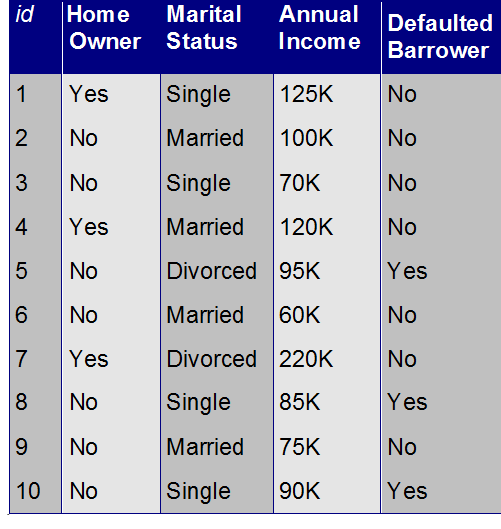
\includegraphics[width=0.8\linewidth,keepaspectratio]{sampledata}
\end{center}
\end{minipage}
}
\hfill
\adjustbox{valign=t}{
\begin{minipage}{0.45\linewidth}
Vocabulary
\begin{itemize}
\item Column-Type: ``attribute'', ``feature'', ``field'', ``dimension'', ``variable''
\item Row-Value: ``instance'', ``record'', ``observation''
\end{itemize}
\end{minipage}
}

\end{frame}


%%%%%%%%%%%%%%%%%%%%%%%%%%%%%%%%%%%%%%%%%%%%%%%%%%%%%%%%%%
\begin{frame}[fragile]\frametitle{Data}	

\begin{itemize}
\item Data Type
\item Data Value
\item Distinctions:
	\begin{itemize}
	\item Same type - different values. Example: height can be measured in feet or meters
	\item Different types  same values. Example: Attribute values for ID and age 
	\end{itemize}
\end{itemize}
\end{frame}


%%%%%%%%%%%%%%%%%%%%%%%%%%%%%%%%%%%%%%%%%%%%%%%%%%%%%%%%%%
\begin{frame}[fragile]\frametitle{Types of Data}	

	\begin{itemize}
	\item {\bf Categorical types (Qualitative):} Nominal and Ordinal
		\begin{itemize}
	\item {\bf Nominal} (numbers do not give sense of order/rank): ID numbers, eye color, zip codes
	\item {\bf Ordinal} (numbers give sense of order/rank): rankings, size in {small, medium, large}
		\end{itemize}
	\item {\bf Numeric types (Quantitative):} Interval and Ratio
			\begin{itemize}

		\item {\bf Discrete:} A discrete attribute has a finite or countably infinite
		set of values. {\bf Binary attributes} are a special case of discrete attributes. 
		\item {\bf Continuous:} A continuous attribute is one whose values are real numbers.
	
	\item {\bf Interval}: calendar dates
	\item {\bf Ratio}: counts, time
			\end{itemize}
	\end{itemize}
NOIR: {\bf N}o {\bf O}il {\bf I}n {\bf R}ivers
\end{frame}

%%%%%%%%%%%%%%%%%%%%%%%%%%%%%%%%%%%%%%%%%%%%%%%%%%%%%%%%%%
\begin{frame}[fragile]\frametitle{Types of Data}	

\begin{itemize}
		\item {\bf Discrete:} A discrete attribute has a finite or countably infinite
		set of values. {\bf Binary attributes} are a special case of discrete attributes. 
		\item {\bf Continuous:} A continuous attribute is one whose values are real numbers.
\end{itemize}
\end{frame}

%%%%%%%%%%%%%%%%%%%%%%%%%%%%%%%%%%%%%%%%%%%%%%%%%%%%%%%%%%
\begin{frame}[fragile]\frametitle{Ordinal}	

	\begin{itemize}
	\item To show relative rankings 
	\item Order matters, but not diff
	\item $Diff(7,5) \neq Diff(5,3)$
	\item ``First is first, however close the second is!!''
	\item Examples: class rank, levels of wellness, 
\item Mohs' Scale of Hardness:	1: Talc,    2:Gypsum,     3:Calcite,      4 :Fluorite

	\end{itemize}

\end{frame}


%%%%%%%%%%%%%%%%%%%%%%%%%%%%%%%%%%%%%%%%%%%%%%%%%%%%%%%%%%
\begin{frame}[fragile]\frametitle{Interval}	

	\begin{itemize}
	\item Diff equal if measured between two equivalent variables
	\item $Diff(100,90) == Diff(90,80)$
	\item Same amount of heat needed to take from 90 to 100 or 80 to 90
	\item Examples: test scores and temperature
	\end{itemize}

\end{frame}


%%%%%%%%%%%%%%%%%%%%%%%%%%%%%%%%%%%%%%%%%%%%%%%%%%%%%%%%%%
\begin{frame}[fragile]\frametitle{Ratio}	

	\begin{itemize}
	\item Clear definition of 0.0; none of a variable at 0.0 (because? there is always `something')
	\item Weight of 8 grams is twice the weight of 4 grams
	\item Example: height, weight, pulse and BP
	\end{itemize}	

\end{frame}


%%%%%%%%%%%%%%%%%%%%%%%%%%%%%%%%%%%%%%%%%%%%%%%%%%%
\begin{frame}[fragile] \frametitle{Discrete Attributes}
\begin{itemize}
\item Finite values
\item Integers
\item Examples: zip codes, counts, \ldots
\end{itemize}
\end{frame}


%%%%%%%%%%%%%%%%%%%%%%%%%%%%%%%%%%%%%%%%%%%%%%%%%%%
\begin{frame}[fragile] \frametitle{Continuous Attributes}
\begin{itemize}
\item Not finite
\item Any level granularity
\item Floating Point numbers
\item Examples: height, temperature, 3.14159\ldots
\end{itemize}

\end{frame}

%%%%%%%%%%%%%%%%%%%%%%%%%%%%%%%%%%%%%%%%%%%%%%%%%%%%%%%%%%
\begin{frame}[fragile]\frametitle{Ordered Data}	

\begin{itemize}
\item Temporal: time based, e.g. retail transaction
\item Sequential: e.g. DNA sequence (ATGC possible letters)
\item Time Series: Series of measurements taken over time. e.g.: financial stock price data
\item Spatial Data: e.g. geographical locations
\end{itemize}
\end{frame}

%%%%%%%%%%%%%%%%%%%%%%%%%%%%%%%%%%%%%%%%%%%%%%%%%%%%%%%%%%
\begin{frame}[fragile]\frametitle{Measures of Similarity and Dissimilarity}

	\begin{itemize}
		\item {\bf Proximity:} either similarity or dissimilarity
			\begin{itemize}
		\item {\bf Similarity:} a numerical measure of likeliness.
		\item{\bf Dissimilarity:} a numerical measure of unlikeliness
		\end{itemize}
		\item {\bf Transformations:} re-parametrize proximity to, say, [0, 1].
\end{itemize}
\end{frame}

%%%%%%%%%%%%%%%%%%%%%%%%%%%%%%%%%%%%%%%%%%%%%%%%%%%%%%%%%%
\begin{frame}[fragile]\frametitle{Similarity and Dissimilarity between Simple Attributes}

		\begin{itemize}
			\item{\bf Nominal:} simple equality test
			\item{\bf Ordinal:} order should be taken into account.
			\item{\bf Ratio:} simple absolute difference of their values.
\end{itemize}
Distance is the measure of similarity-dissimilarity.
\end{frame}

%%%%%%%%%%%%%%%%%%%%%%%%%%%%%%%%%%%%%%%%%%%%%%%%%%%%%%%%%%
\begin{frame}[fragile]\frametitle{Euclidean distance} 
$d(a,b) = \sqrt{\sum_{k=1}^{n} (a_k - b_k)^{2}}$
\end{frame}

%%%%%%%%%%%%%%%%%%%%%%%%%%%%%%%%%%%%%%%%%%%%%%%%%%%%%%%%%%
\begin{frame}[fragile]\frametitle{Minkowski distances}

$d(a,b) = \left(\sum_{k=1}^{n} |a_k - b_k|^{r}\right) ^{1/r}$

	\begin{itemize}
		\item {\bf r = 1} City block (Manhattan, taxicab, $L_{1}$ norm) distance.
		\item {\bf r = 2} Euclidean distance ($L_{2}$ norm).
		\item {\bf r = $\infty$} Supreme ($L_{max}$ or $L_{\infty}$) distance. Here r is not put equal to $\infty$ but tends to or limit to $\infty$
\end{itemize}

Considering this formula for finding norm (ie length, or tcan be same as length of diff between a and b):

	\begin{itemize}
		\item Putting a very large number, say, 1000, for $v=[0 1 10]$, the norm would be $(0^1000 + 1^1000 + 10^1000)^{1/1000}$. 
		\item Here the last number becomes very big, but its 1000th root gives the same number as answer ie 10. 

		\item So, this method biases towards large numbers.
\end{itemize}
		
\end{frame}

%%%%%%%%%%%%%%%%%%%%%%%%%%%%%%%%%%%%%%%%%%%%%%%%%%%
\begin{frame}[fragile] \frametitle{Visualizing Norms}


Vectors having:

	\begin{itemize}
		\item Euclidean distance Norm as 1, when plotted look like circle.
		\item Manhattan distance as Norm as 1, when plotted makes a inner Square.
		\item Minkowski distance with $r=\infty$ norm as 1, when plotted looks outer Square.
				\item Minkowski distance with smaller $r$ norm as 1, when plotted looks somewhere between.
\end{itemize}

\begin{center}
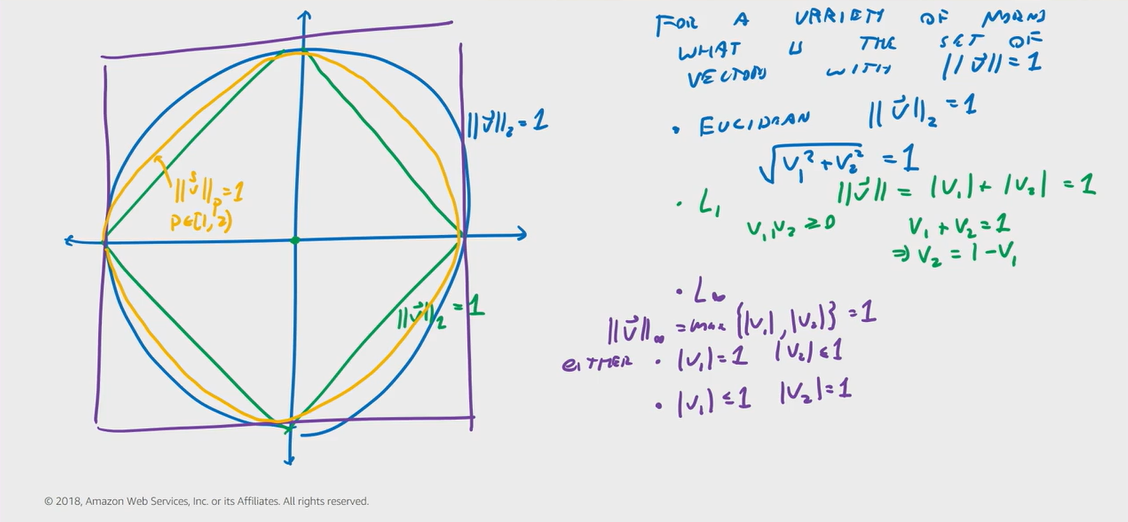
\includegraphics[width=0.6\linewidth,keepaspectratio]{awsmaths1}
\end{center}

{\tiny (Ref: Math for Machine Learning - Brent Werness, AWS)}

\end{frame}


%%%%%%%%%%%%%%%%%%%%%%%%%%%%%%%%%%%%%%%%%%%%%%%%%%%%%%%%%%
\begin{frame}[fragile]\frametitle{Properties Euclidean distances}

		\begin{itemize}
			\item {\bf Positivity}
			\begin{itemize}
				\item d(a,b) $\geq$ for all a and b,
				\item d(a,b) = 0 only if a = b
			\end{itemize}
			\item {\bf Symmetry} \\
				d(a,b) = d(b,a) for all a and b
			\item {\bf Triangle Inequality} \\
				d(a,c) $\leq$ d(a,b) + d(b,c) for all points a, b, and c
\end{itemize}
\end{frame}


%%%%%%%%%%%%%%%%%%%%%%%%%%%%%%%%%%%%%%%%%%%%%%%%%%%%%%%%%%
\begin{frame}[fragile]\frametitle{Metrics}

	Measures that satisfy all three properties are known as metrics.

	\begin{table}[!h]
		\centering
		\begin{tabular}{| l | l | l |}
			\hline
			point & x coordinate & y coordinate \\ \hline
			p1 & 0 & 2 \\ \hline
			p2 & 2 & 0 \\ \hline
			p3 & 3 & 1 \\ \hline
			p4 & 5 & 1 \\ \hline
		\end{tabular}
		\begin{tabular}{| l | l | l | l | l |}
			\hline
			 & p1 & p2 & p3 & p4 \\ \hline
			p1 & 0.0 & 2.8 & 3.2 & 5.1 \\ \hline
			p2 & 2.8 & 0.0 & 1.4 & 3.2 \\ \hline
			p3 & 3.2 & 1.4 & 0.0 & 2.0 \\ \hline
			p4 & 5.1 & 3.2 & 2.0 & 0.0 \\ \hline
		\end{tabular}
		\caption{(a) x and y coordinates, (b) Euclidean distance matrix}
\end{table}
\end{frame}


%%%%%%%%%%%%%%%%%%%%%%%%%%%%%%%%%%%%%%%%%%%%%%%%%%%%%%%%%%
\begin{frame}[fragile]\frametitle{Metrics}

	Measures that satisfy all three properties are known as metrics.

\begin{table}[!h]
		\centering
		\begin{tabular}{| l | l | l | l | l |}
			\hline
			$L_{1}$ & p1 & p2 & p3 & p4 \\ \hline
			p1 & 0.0 & 4.0 & 4.0 & 6.0 \\ \hline
			p2 & 4.0 & 0.0 & 2.0 & 4.0 \\ \hline
			p3 & 4.0 & 2.0 & 0.0 & 2.0 \\ \hline
			p4 & 6.0 & 4.0 & 2.0 & 0.0 \\ \hline
		\end{tabular}
		\begin{tabular}{| l | l | l | l | l |}
			\hline
			$L_\infty$ & p1 & p2 & p3 & p4 \\ \hline 
			p1 & 0.0 & 2.0 & 3.0 & 5.0 \\ \hline
			p2 & 2.0 & 0.0 & 1.0 & 3.0 \\ \hline
			p3 & 3.0 & 1.0 & 0.0 & 2.0 \\ \hline
			p4 & 5.0 & 3.0 & 2.0 & 0.0 \\ \hline
		\end{tabular}
		\caption{(a) $L_{1}$ distance matrix, (b) $L_{\infty}$ distance matrix}
\end{table}
\end{frame}

%%%%%%%%%%%%%%%%%%%%%%%%%%%%%%%%%%%%%%%%%%%%%%%%%%%%%%%%%%%
%\begin{frame}[fragile]\frametitle{Similarities between Data Objects}
%	If s(x,y) is the similarity between points x and y, then the typical properties
%	of similarities are the following:
%		\begin{itemize}
%			\item s(x,y) = 1 only if x = y. (0 $\leq$ s $\geq$ 1)
%			\item s(x,y) = s(y,x) for all x anf y. (Symmetry)
%\end{itemize}
%\end{frame}


%%%%%%%%%%%%%%%%%%%%%%%%%%%%%%%%%%%%%%%%%%%%%%%%%%%%%%%%%%
\begin{frame}[fragile]\frametitle{Examples: Similarity Measures of Binary Data:}

	Have values between 0 and 1.
	
	Let a and b be two objects that consist of n binary attributes 
	
	i.e., two binary vectors
	
	Possibilities:

		$f_{00}$ = the number of attributes where a is 0 and b is 0 \\
		$f_{01}$ = the number of attributes where a is 0 and b is 1 \\
		$f_{10}$ = the number of attributes where a is 1 and b is 0 \\
		$f_{11}$ = the number of attributes where a is 1 and b is 1 \\
\end{frame}

%%%%%%%%%%%%%%%%%%%%%%%%%%%%%%%%%%%%%%%%%%%%%%%%%%%%%%%%%%
\begin{frame}[fragile]\frametitle{Examples: Simple Matching Coefficient (SMC)} 

$
		SMC = \frac{number\;of\;matching\;attribute\;values}{number\;of\;attributes} = 
		\frac{f_{11} + f_{00}}{f_{01} + f_{10} + f_{11} + f_{00}}
$
\end{frame}

%%%%%%%%%%%%%%%%%%%%%%%%%%%%%%%%%%%%%%%%%%%%%%%%%%%%%%%%%%%
%\begin{frame}[fragile]\frametitle{Examples: Jaccard Coefficient}
%To handle objects consisting of 
%
%
%$
%			J = \frac{number\;of\;matching\;presences}{number\;of\;attibutes\;not\;involved\;in\;00\;matches} =
%			\frac{f_{11}}{f_{01} + f_{10} + f_{11}}
%$
%\end{frame}

%%%%%%%%%%%%%%%%%%%%%%%%%%%%%%%%%%%%%%%%%%%%%%%%%%%%%%%%%%
\begin{frame}[fragile]\frametitle{Examples: Cosine Similarity} 

$
		cos(a,b) = \frac{a . b}{\|a\| \|b\|} = \frac{\sum a_{i}. b_{i}}{\sqrt{\sum(a_{i})^2} .  \sqrt{\sum(b_{i})^{2}}}
$
\end{frame}

%%%%%%%%%%%%%%%%%%%%%%%%%%%%%%%%%%%%%%%%%%%%%%%%%%%%%%%%%%%
%\begin{frame}[fragile]\frametitle{Examples: Extended Jaccard Coefficient} 
%
%		\begin{equation}
%			EJ(a,b) = \frac{a*b}{\|a\|^{2} + \|b\|^{2} - a*b}
%\end{equation}
%\end{frame}

%
%%%%%%%%%%%%%%%%%%%%%%%%%%%%%%%%%%%%%%%%%%%%%%%%%%%%%%%%%%%
%\begin{frame}[fragile]\frametitle{General Characteristics of Data Sets}
%
%			\begin{itemize}
%				\item {\bf Dimensionality:} number of attributes 
%				\item {\bf Sparsity:} asymmetric features, most
%				are 0.
%				\item {\bf Resolution:}  the surface of the Earth seems very uneven at a resolution of a few meters, but is *
%				relatively smooth at a resolution of ten kilometers. Intra-day-Intra-hour tracking.
%\end{itemize}
%\end{frame}
%
%%%%%%%%%%%%%%%%%%%%%%%%%%%%%%%%%%%%%%%%%%%%%%%%%%%%%%%%%%%
%\begin{frame}[fragile]\frametitle{Type of Data Sets}
%
%		\begin{itemize}
%			\item {\bf Records:} Data-matrix, Transaction data 
%			\item {\bf Graph:} Social Networks
%			\item {\bf Ordered:} Sequential Data (temporal data), Time Series Data, Spatial Data
%\end{itemize}
%\end{frame}
%
%%%%%%%%%%%%%%%%%%%%%%%%%%%%%%%%%%%%%%%%%%%%%%%%%%%%%%%%%%%
%\begin{frame}[fragile]\frametitle{Record Data}
%
%		\begin{itemize}
%				\item {\bf Transactions:} each record involves a set of items. 
%				\item {\bf The Data Matrix:} same fixed set of numeric attributes.
%				\item {\bf The Sparse Data Matrix:} many zeros, few non-zeros
%\end{itemize}
%\end{frame}
%
%%%%%%%%%%%%%%%%%%%%%%%%%%%%%%%%%%%%%%%%%%%%%%%%%%%%%%%%%%%
%\begin{frame}[fragile]\frametitle{Graph-Based Data}
%			\begin{itemize}
%				\item Data objects are mapped to nodes of the graph
%				\item Relationships among
%				objects are captured by the links between objects and link propeties. 
%\end{itemize}
%\end{frame}
%
%%%%%%%%%%%%%%%%%%%%%%%%%%%%%%%%%%%%%%%%%%%%%%%%%%%%%%%%%%%
%\begin{frame}[fragile]\frametitle{Ordered Data}
%			\begin{itemize}
%				\item {\bf Sequential Data (temporal data):} Each record has a time associated with it. 
%				\item {\bf Sequence Data:} such as a sequence of words or letters. 
%				\item {\bf Time Series Data:} on a time series (equal intervals)
%				\item {\bf Spatial Data:} have spatial attributes, such as positions
%\end{itemize}
%\end{frame}

